%databaseimpl.tex
The implementation of the MySQL database is done in MySQL Workbench 5.2.40 which is a GUI tool that provides a large set of features for various purposes.

Due to the dependencies of the various tables, the order of how the need to be created is quite strict. 
The code to create the tables is found in the appendix \autoref{MySQLcode}. To make sure the ``username'' and ``userID'' follows the previously stated rules, both fields has been made \verb+UNIQUE NOT NULL+ and the ``userID'' furthermore has \verb+AUTO_INCREMENT+ as seen in \autoref{createAuthUsers}. This makes sure there can be no one with the same ``username'' or ``userID'' and the ``userID'' will automatic increase when new data is inserted. 
This also guarantees a one-to-one relation between both ``Profile'' and ``AuthUsers'' and ``Departments'' and ``AuthUsers''. To be able to distinguish between ``Department'' and ``Profiles'' a filed called \verb+aRole+ is used. 
This is a int and will hold a number, which will be used at software level to do the distinguishing. The same applies for the distinguishing in ``Profile'' (code shown in \autoref{createProfile}), here a field called \verb+pRole+ holds an int, which again will be used at software level.

The MySQL Workbench provides the functionality to create a ERR diagram form an existing database, this diagram is shown in \autoref{fig:workbenchRight}. The diagram is con completely as MySQL workbench creates it, the real is shown in the appendix \autoref{errDiagram}. But this is a error in the software; as seen in the diagram, the tool generates the ``Profiles''$\rightarrow$''AuthUsers'' as a one-to-many relation. This however, is not possible since the ``idUser'' field in ``AuthUsers'' is unique (as seen in \autoref{createAuthUsers}), the same goes for both ``Departments'' and ``Medias''.

\begin{figure}
	\centering
		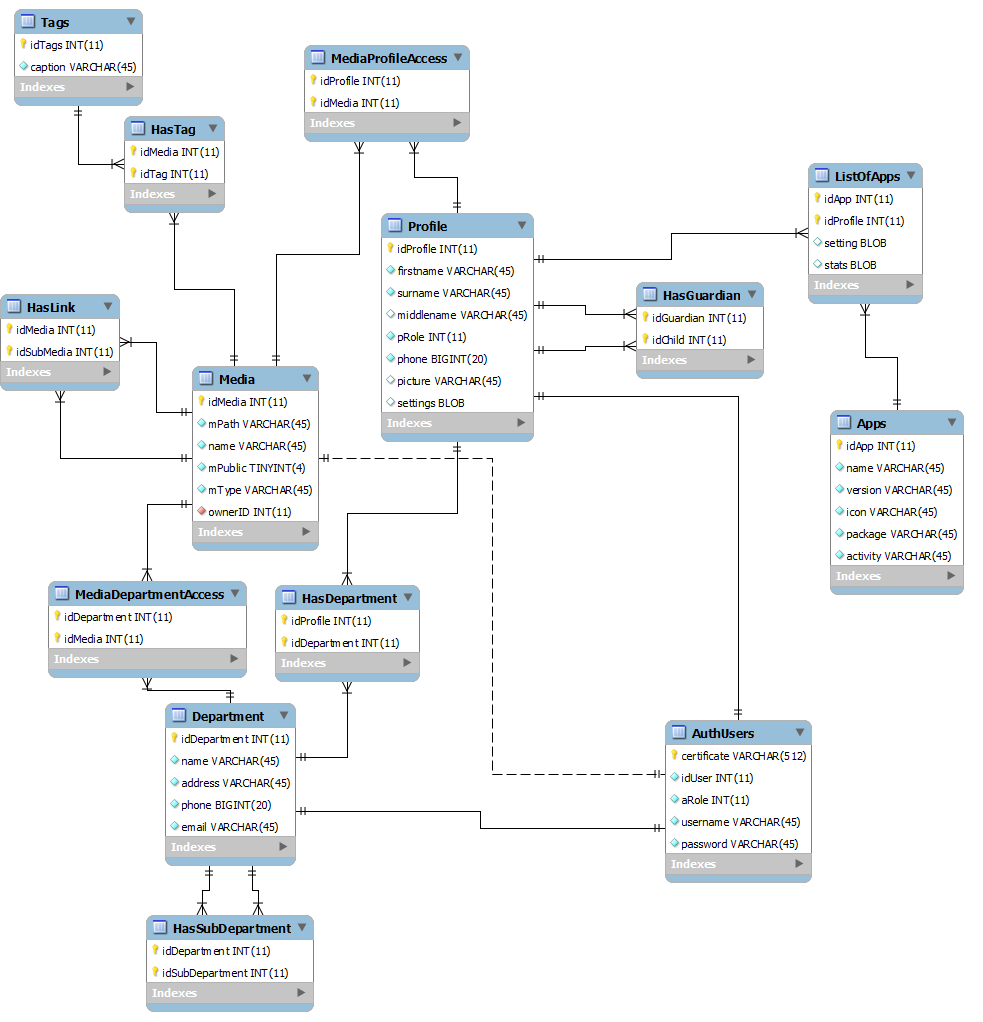
\includegraphics[width=1.00\textwidth]{images/workbenchRight.png}
	\caption{The ERR diagram}
	\label{fig:workbenchRight}
\end{figure}


To make the deletion of data easy, many of the filed in the tables has the constraint \verb+ON DELETE CASCADE+. This can be ``dangerous'', as side-effects can result in unintended data will be deleted. To makes sure no unintended data will be deleted, the software level implementation needs to warn the user when deleting data. Furthermore an analysis has been made to argue for which fileds can have this constraint. The following tables and fields has the cascade constraint: 
\begin{verbatim}
``Profiles''.''idProfile'', 
``ListOfApps''.''idProfile'', 
``HasDepartment''.''idProfile'', 
``HasGuardian''.''idGuardian'', 
``HasGuardian''.''idChild'', 
``Media''.''OwnerID'', 
``HasTag''.''idMedia'', 
``HasLink''.''idMedia'', 
``HasLink''.''idSubMedia'',
''MediaProfileAccess''.''idProfile''.
\end{verbatim}

\subsubsection*{Use case}
 An use case of the constraint is:
\begin{quotation}
``A user ``Jesper'' wishes to delete his entire profile''
\end{quotation}
What will happen is:
\begin{enumerate}
	\item A deletion of the ``userID'' in ``AuthUsers'' is executed
	\item The relation between ``AuthUsers'' and ``Profiles'' will delete the profile
	\item The relation between ``Profiles'' and ``HasGuardian'' will delete all fields where the ``userID'' is either ``idGuardian'' or ``idChild''
	\item The relation between ``AuthUsers'' and ``Media'' will delete all fields where ``idUser'' is the owner
	\item The relation between ``Media'' and ``HasTag'' will delete all fields where ``HasTags''.``idMedia'' equals ``idMedia''
	\item The relation between ``Media'' and ``HasLink'' will delete all fields where ``HasLink''.''idMedia'' or ``HasLink''.''idSubMedia'' equals ``idMedia''
\end{enumerate}

